\chapter{Alloy Specification Framework}\label{c:alloy}

As aforementioned, this dissertation aims to tackle the security vulnerabilities resulted from the miss-configuration over ROS files. In this chapter, it is intended to explore the Alloy framework that is relevant to overcome the above-mentioned challenge. % as well as previous developed work that has the same or similar goals as this thesis (\ref{s:alloy-relWork}).

The increasing usage of robotics onto safety-critical systems results in demanding considerations over ensuring the proper correctness of both software and hardware, as failures often leads to fatal consequences, especially regarding the security domain. Thus, the use of formal methods and verification techniques, especially in systems highly reliant on flexibility and reliability, is recommended to avoid security-critical faults \cite{clarke2011model}. Software frameworks designed for this purpose must provide methods to perform structural design over systems with rich structures, abstracting their behaviour as a conventional model. Additionally, these frameworks must support features to enable automate analysis, in which property evaluation over these designed models is used as technique. 

The \textit{Alloy Framework} \cite{alloy-DJ}, fits within this context, as it furnishes a declarative relation-based language, used for software modelling, complemented with extended tools supporting analysis over these models \cite{alloy-6}. The language combination of both \textit{Relational} and \textit{Linear Temporal Logic} (LTL) enables the ability to model both systems with rich structures and complex behaviour. To address the correctness over the specified model, Alloy performs model-checking techniques over these logic languages, where the model $M$ is exhaustively checked over property verification \cite{lwspecification}.

The framework \textit{analyzer} takes the specified model's restrictions into account, performing \textit{Bounded} and \textit{Unbounded} Model Checking to find instances that satisfy those implied restrictions. It can be also be useful for checking model properties, where the analyzer will try to return a counterexample instance. Instances are displayed by the framework Visualizer, alongside with the modelling process steps, regarding a trace representation. Instances appearance can be customized, using the \textit{theme}'s extension \cite{alloy-6}.

This chapter will go through these principles in further depth, to give the reader a proper review on how Alloy is structured, as its importance as a model checker to the computation domain, supported by a previously configured example where ROS communication architecture is structurally modelled. Since system analysis rely on the reasonable implementation of Model-Checking techniques, the following section within this subject intends to cover a clear contextualization on this matter. % since it is highly important on understanding how Alloy's verification process works.

\section{Model Checking}

% Model-checking is increasingly popular in the early phases of the software development process. To establish the cor- rectness of a software design one must usually verify both structural and behavioral (or temporal) properties. Unfor- tunately, most specification languages, and accompanying model-checkers, excel only in analyzing either one or the other kind. This limits their ability to verify dynamic systems with rich configurations: systems whose state space is character- ized by rich structural properties, but whose evolution is also expected to satisfy certain temporal properties. To address this problem, we first propose Electrum, an extension of the Alloy specification language with temporal logic operators, where both rich configurations and expressive temporal properties can easily be defined. Two alternative model-checking techniques are then proposed, one bounded and the other unbounded, to verify systems expressed in this language, namely to verify that every desirable temporal property holds for every possible configuration.

Performing software testing has been regarded as the established assessment procedure in which functional and non-functional specifications are evaluated. The conventional approach on software verification is based on testing the system with different inputs, to achieve quality assurance over several intended specifications \cite{beyer2017software, briand2001uml}. As this technique demands exhaustively evaluation over pre-selected test data, it is commonly explored over automated tools, since manual testing is time-consuming and prone to errors \cite{clarke1976program, fraser2009testing}.

% Model-based testing arises as a viable alternative technique, in which both test cases and intended behaviour relies on the design of an abstract mode, presenting remarkable benefits to the latter approach. \cite{apfelbaum1997model} Thus, to perform full verification over systems, the \textit{model-checking} technique can be used to automatically interpret counterexamples as test cases, consequently enabling far better degrees of coverage than conventional testing. \cite{fraser2009testing, beyer2017software}

\textit{Model Checking} presents itself as a novel technique with the purpose of verifying temporal properties over the system finite-state, with the latter being duly represented as a conclusive model. Additionally, it enables \textit{model-based testing} by automatically interpreting counterexamples as test cases, resulting in significantly greater degrees of coverage than conventional testing \cite{fraser2009testing, beyer2017software}. This technique is becoming highly used due to its importance as an early phase approach upon developing systems \cite{lwspecification}, as it confers the most valued functionality over model-checking frameworks, in which concrete models, regarding the software architecture, is exhaustively checked over behavioural properties. 

It provides highly automatic verification procedures, where other techniques, such as theorem provers fails to address, due to its deductive reasoning nature. The representation of not satisfied specifications over counterexamples, confers great functionality to this technique, often required for debugging matters.
However, the system's inevitable state expansion consequently causes the complexity increase on verification. This is referred to as the \textit{state explosion problem}, in which model-checking is unable to handle the size of the state space \cite{clarke2011model, clarke1997model}. Yet, this is can be mitigated using bounded techniques.

Model Checking techniques accounts property verification of systems through the implicit use of temporal logic to express \textit{dynamic} behaviour through the course of the system evolution. Thus, the system must be abstractly represented as a transition system, perceived as concrete models, to perform property checking over the latter, while considering the formula defined in a temporal logic \cite{huth2004logic, vakili2012temporal}. 

\vspace{0.5cm}
\textbf{Transition System}

A \textit{Transition System} is defined over a graph-based structure, that confers additional representation over the mathematical graph structure. The latter offers weak ability to provide a concrete system description over a discrete model. Commonly, transition system confers a labelling function that maps each state, naturally perceived as graph node, with so-called \textit{atomic propositions}. These propositions evaluate system variables in each state \cite{muller1999model, vakili2012temporal}.

\textit{Kripke Structures} were intentionally conceived to address the model checking field of action, so they naturally fall under the umbrella of this vast domain \cite{muller1999model}.

Conceptually, a \textit{Kripke Structure} defines a model $M$ with the following tuple structure $M = (S,I,R,p,L)$, where: $S$ is a finite set of states; $I$ represents a set of initial states, so naturally $I$ is a subset of $S$ ($I \subseteq S$); $r$ defines the \textit{transition relation} as it accounts the transitions between states; $L$ is an \textit{interpretation} that defines the labelling function; Accordingly, it assigns each state with a set of valid atomic propositions $p_{s}$ enjoyed by it, draw from the domain of $p$ ($p_{s} \subseteq p$). 

\vspace{0.5cm}

Model Checking is a \textit{model-based} technique in which property verification concerns are centered on the concept of \textit{satisfaction}. Therefore, the corresponding model-checker must be capable of checking if the model $M$ satisfies a desirable property, expressed as temporal logic formula $\psi$. As this computing process relies on a state representation, the formula verification also accounts a model state $s$. $M,s \models \psi$ \cite{huth2004logic, muller1999model}.

Additionally, the semantics of the temporal logic relies on how the latter addresses time as an evolving approach towards state verification. Notably, temporal logics are either qualified as \textit{linear-time} or as \textit{branching-time} \cite{huth2004logic}. In the former approach, time is perceived as linear path and the corresponding transition system is abstracted by a set of infinite traces. The latter denotes time as a branching model, in which the transition system is abstracted by a set of infinite computation trees, consequently enabling non-deterministic considerations about the system evolution. The choice on the logic semantics relies on the system properties to be analyzed \cite{muller1999model}, as they confer different model-checking algorithms \cite{huth2004logic}. 


% \subsection{Model Checking in Alloy}
% 
% Following the temporal logic semantics, Alloy specification language embeds the linear temporal logic into the first-order logic, thus, it makes use of both temporal and relational quantifiers to properly express behavioural verification over time \cite{lwspecification}. \textit{First-Order Temporal Logics} present additional techniques for reasoning about behaviour, while accounting the basis of the first-order logic, that usually confers the capability to express the well-formedness of the system structure \cite{lwspecification, konur2010survey}.
% 
% The \textit{FOLTL} syntax confers bounded and unbounded semantics, in which 
% 
% The Alloy Framework performs model checking through \textit{2} distinct techniques, those being the \textit{Bounded} and \textit{Unbounded}, already introduced earlier in this section, to verify that temporal properties hold considering the model specification \cite{lwspecification}. 
% 
% Usually, the \textit{Bounded} model checking is considered as first approach to validate the model specification. In addition, performing \textit{Unbounded} model checking proves to be a novel approach to check the model consistency, as it provides high degrees of reliability due to its verification coverage. 

\section{Structural Design}

The \textit{Alloy framework} presents itself as a formal modelling language, conceived to properly address model-checking techniques over their specification language, where both structural design and temporal behaviour, naturally specified over properties, can easily be defined. Formerly, Alloy was inherently static \cite{lwspecification}, meaning that it only excel the structural design, where its language was based on first-order logic. The analysis process relied on a bounded model checking technique with no support for temporal behaviour. Notwithstanding, the latest release of Alloy confers the ability to properly deal with expressive temporal properties, as well as trace evaluation over time, while employing the former structural approach. 

As intentionally design to formally abstract both system's configuration and behaviour, Alloy successfully incorporates a set of features, within a well-documented and wide-ranged syntax that consequently allows large specification development \cite{lwspecification}. The following subsection \ref{c:alloy-sm} addresses the Alloy concepts required for understanding how system modelling is covered. 

\subsection{Structural Modelling}\label{c:alloy-sm}

Alloy aims to address the complexity behind richly structured systems, that require critical control over their intended behaviour, by presenting a novel approach for abstracting these systems as conventional models. 

System's structures can be specified over time-evolving states, where its behaviour clearly identifies the states' inbetween transitions. The conception of system transitioning offers a great formal approach when it comes to reason about the system's design.

The Alloy structural definition relies on a relation way of connecting system's elements, where the latter is abstracted in terms of relations. In Alloy, unary relations, commonly known as sets, are labelled as \textit{signatures}, that are inhabited by a set of \textit{atoms}, from a finite universe of discourse. Atoms are perceived as the lowest-grain elements, with no particular semantics attached. A signature, identified by the keyword $sig$, might include multiple \textit{field} declarations enclosed between braces, addressing relation between the signature's atoms and a set or other relation. Fields are inhabited by tuples of atoms from the universe, that must meet the same arity.

Signatures can either be perceived as a top-level signature, or as other signature's subset. Signature hierarchy is conceivable through disjoint extensions ($extends$), or by set inclusion ($in$). The $abstract$ keyword declares a signature that contains no atoms beyond those within its extensions. 

To address default configuration over the universe's multiplicity, both signatures and fields can be specified under a multiplicity constraint. The former constrains the number of signature atoms, where it is commonly used to express singleton sets, over the constraint keyword $one\ sig$. Fields, however, makes great use of multiplicities by restricting behaviour over relations between atoms. In addition to these model constraints, explicitly specified over the course of the modelling process, system assumptions can be defined over axioms, expressed as $facts$, where multiple constraints can be incorporated \cite{gheyi2007formally}.

Moreover, the latest Alloy version enables evaluation changing throughout the trace evolution, consequently allowing the consideration of both signatures and fields as time mutable declarations, through the usage of the keyword $var$.

Throughout the sections that follow, it will be presented an illustrative example over which graph theory rests, this being the study of \textit{Eulerian Circuits}. This example will be used to duly contextualize both modelling and verification process in Alloy. \textit{Eulerian Circuits} must meet several behaviour constraints over the classic graph definition, that must be addressed over model constraints. However, the structural modelling must be provided beforehand.

\subsubsection{Model Structure}

With regard to the presented example, as it falls under the study of graphs theory \cite{west2001introduction}, it follows an abstract representation of the graph mathematical structure. In this sense, a graph is made up of nodes which are connected by edges. 

Considering the Alloy's abstract ability to reduce complexity over model designing, at a high degree of abstraction, graphs can be represented as a set of \textit{nodes}, that connect together over relations, with no need to address edges as a separated structure declaration. 

\begin{lstlisting}[title={Graph representation over a sigle Node declaration.}, otherkeywords = {abstract, sig, module, var, set, fact, extends, no, in}, label={lst:node},floatplacement=H]
sig Node {
    adj : set Node, 
    var visited : set Node
}
\end{lstlisting}

As depicted above, the $sig$ keyword followed by the corresponding \textit{Node} signature declaration, represents the state of our intended example. The \textit{Node} signature is defined by a static set of node \textit{atoms}, that combined denotes the finite universe of discourse.

Then, \textit{fields} are enclosed between braces upon the \textit{Node} signature declaration. The \textit{adj} concerns the graph edges, where each node can be connected to a set of nodes. As it is identified as an immutable \textit{field}, the corresponding relation between atoms is static. Moreover, addressing additional graph functionality, it is desirable to concern about the visited nodes. The latter represents a mutable relation, identified by the keyword $var$, meaning that its evaluation may change during the course of the trace's evolution, as opposed to the static ones. 

Relation multiplicity constraints are explicitly defined in the field declaration through the use of multiplicity operators, with those being $one$, $lone$, $some$ and $set$.

\begin{figure}[H]
    \centering
    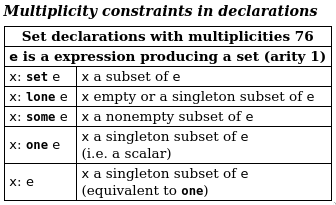
\includegraphics[width=0.4\linewidth]{img/alloy_multiplicity.png}
    \caption{Alloy Multiplicity constraints. Extracted from \cite{alloy-qr}.} 
    \label{fig:alloy-multiplicity}
\end{figure}


Structural constraints can be entailed over explicitly signature declaration. These are often referred as \textit{signature facts}, universally quantified over the signature's set \cite{alloy-qr}. Suppose a hypothetical design scenario, where the relation \textit{adj} is labelled as mutable. To ensure that the graph architecture consistency, in which, edges are structurally fixed, the following constraint can be specified. Additionally, consider the following \textit{graph} property, where it is desirable to express the following axiom: \textit{The graph contains no self-loops.}

\begin{lstlisting}[title={\textit{Node} hypothetical constraints over the signature definition.}, otherkeywords = {abstract, sig, module, var, set, fact, extends, no, in, this, not, always, \', \=}, floatplacement=H]
sig Node {
    var adj : set Node, 
    var visited : set Node
} {
    always adj' = adj
    this not in adj
}
\end{lstlisting}

As stated, the former poses a model incoherence within the \textit{Node} signature declaration, as \textit{adj} field is formerly labelled as mutable, that is later refuted by specifying $always \ adj'\ =\ adj$. This latter introduces the Alloy language's ability to express temporal behaviour through these \textit{two} \textit{linear temporal logic} operators, $'$ and $always$ respectively. 

\begin{figure}[H]
    \centering
    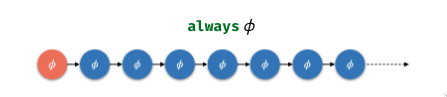
\includegraphics[width=0.7\linewidth]{img/alloy_always.png}
    \caption{$always$ behavioural representation.}
    \label{fig:alloy-always}
\end{figure}

The $always$ operator expresses a universal quantifier over time, imposing a constraint throughout the trace. The $'$ operator evaluates the \textit{adj} relation in the next state. So, the formula specifies that the evaluation of \textit{adj} in the next state is always the same of the current state. Alloy integrates LTL into the standard Relational logic, therefore, supporting both linear temporal logic unary and binary modal operator.

Whereas the latter expresses the \textit{no self-loop} graph property. Even though \textit{adj} is introduced as a relation between \textit{Nodes}, it is perceived as a set of \textit{Nodes} due to specification with the signature declaration. The keyword $this$ addresses each \textit{Node} atom, as self representation of the considered atom. The remaining specifies the intended behaviour, as it specifies the non-inclusion ($not\ in$) over the set of its adjacent nodes.

% The considered property expressness has a high level of complexity attached, and can be easily simplified over \textit{this not in adj}, as they both hold the same value. However, for contextualization reasons, and to introduce to the reader multiple Alloy's operators, the above is taken into account.

Aside from the structural constraints implied within signature's declaration, multiplicity over fields \ref{fig:alloy-multiplicity} and signatures also narrows the model's universe. The field multiplicity operators could be used to limit the number of signature atoms. Despite this, signature multiplicity is frequently used to represent singleton $one\ sig$ sets.

\begin{lstlisting}[title={\textit{Node} signature hierarchy.}, otherkeywords = {one, abstract, sig, module, var, set, fact, extends, no, in}, floatplacement=H]
one sig Init extends Node {}
var one sig Euler in Node {}
\end{lstlisting}

The above signatures accurately support the \textit{Eurelian} circuit concept. An \textit{Eurelian} path denotes a trail in a finite graph where every edge is visited exactly once. Additionally, an \textit{Eurelian} circuit implies that the path must start and end at the same node, denoted as \textit{Init}. As this latter differs from the remaining \textit{Node} atoms, the $extends$ keyword must be used to imply hierarchy disjointness. The \textit{Euler} node is an abstract representation of the current node that is being visited. As this impose a mutable state ($var$) over nodes, hierarchy disjointness is not appropriate. Hence, to properly model that the \textit{Euler} node can be included in an arbitrary atom, signature inclusion ($in$) should be used.

Both signatures are preceded by the $one$ keyword, imposing a multiplicity constraint over each signature declaration. Setting the multiplicity to $one$ means that each assessed model instance must have precisely one \textit{Init} atom and one \textit{Euler} atom. It should be noted that, since the \textit{Node} declaration is not preceded by the $abstract$ keyword, its atoms do not solely belong to the \textit{Init} signature. 

Additional modelling constraints can be specified by making use of the $fact$ declaration. The formula specified inside each $fact$ declaration denotes a model axiom, that holds a truth model assumption, to serve as a premise for further reasoning. 

The \textit{Eulerian} path denotes a trail within a finite graph, with each graph edge being visited precisely once. Thus, this already implies that the graph must be connected, where each node must be reachable, and undirected, where edges are non-oriented.

\begin{lstlisting}[title={Graph restrictions through $fact$ declaration.}, otherkeywords = {abstract, sig, module, set, fact, iden, no, in, \=, \*, \+, \~, \-\>, \&}, floatplacement=H]
fact eulerian_considerations {
    adj = ~adj
    no iden & adj
    Node->Node in *(adj + ~adj)
}
\end{lstlisting}

These expressions, above specified, make use of some valued Alloy operators, consequently identified either as a set-theory operator or as a relational operator. Despite the extensive number of operators supplied by Alloy's language, every expression, through the usage of \textit{FOL} quantifiers and \textit{LTL} operators, is later translated to boolean-based expressions. 

\begin{figure}[H]
    \centering
    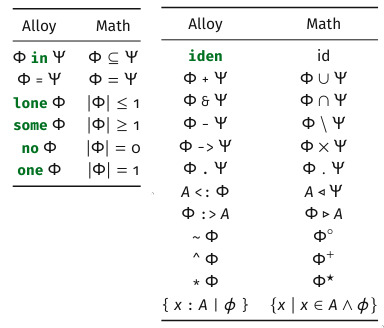
\includegraphics[width=0.5\linewidth]{img/alloy_relational_logic.jpg}
    \caption{Relational Logic Syntax.}
    \label{fig:alloy-rel}
\end{figure}

Regarding set-theory, set intersection (denoted by $\&$) and set conjunction (denoted by $+$) are introduced. The remaining are relational based operators. The $\sim adj$ denotes the converse relation of \textit{adj}, and the $\rightarrow$ represents the Cartesian product operator. The reflexive transitive closure operator ($\ast$) confers the
smallest transitive $\ast(adj\ +\ ~adj)$ relation containing all the identifiers, reachable in zero or more steps, through the implicit use of the set composition operator ($\cdot$). The other transitive closure $\string^$ is defined as $\string^ rel\ =\ \ast rel\ -\ iden$.

\begin{figure}[H]
    \[\string^ rel\ =\ rel\ + rel \cdot rel\ +\ rel \cdot rel \cdot rel\ + ... \]  
\caption{Reflexive transitive closure operator.}
\label{math:alloy-transitive}
\end{figure}

\subsubsection{Everything is a Relation}

As previously stated, Alloy emphasizes the mathematical relation concept to describe systems as a conventional designed model, through conceiving a set $R$ of relations. Moreover, Alloy confers the ability to express their relations as \textit{variable} \cite{lwspecification}. An Alloy relation presents itself as a set of tuples of \textit{atoms} drawn from the same universe context. Subsequently, each relation tuple must meet the same arity of the relation \cite{alloy-docs}.

The \textit{Alloy Evaluator} \cite{alloy-6} confers additional functionality to the \textit{Visualizer}. It allows the user to type Alloy-based expressions against the existing model, used to gather structure information about the existing model \cite{alloy-docs}. In the Figure \ref{fig:alloy-evaluator_1} is presented both \textit{Node} signature and \textit{adj} relation, regarding the model depicted in the Figure \ref{fig:alloy-eulerian_1}.

\begin{figure}[H]
    \centering
    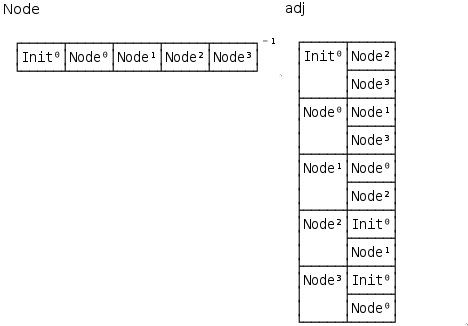
\includegraphics[width=0.5\linewidth]{img/alloy_evaluator1.png}
    \caption{\textit{Node} and \textit{adj} relations.}
    \label{fig:alloy-evaluator_1}
\end{figure}

Additionally, the use of the relational based operators $<:$ and $:>$ denote explicit restriction over relations, with the former restricting its domain, and the latter restricting its range.

\begin{figure}[H]
    \centering
    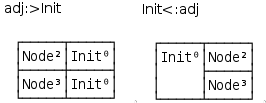
\includegraphics[width=0.4\linewidth]{img/alloy_evaluator2.png}
    \caption{\textit{Init} adjacent nodes.}
    \label{fig:alloy-evaluator_2}
\end{figure}


In order to prevent unwanted model structural scenarios, the intended model can be visualized over the \textit{Alloy Visualizer}, upon executing the $run$ analyzing command. In the Figure \ref{fig:alloy-eulerian_1} is depicted an instance of an acceptable configuration of the \textit{Eulerian} circuit with \textit{5 Node} atoms, since every model constraint was duly specified.

\begin{figure}[H]
    \centering
    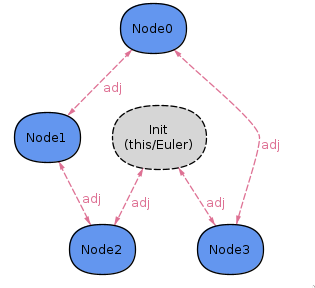
\includegraphics[width=0.5\linewidth]{img/alloy_eulerian_1.png}
    \caption{Acceptable \textit{Eulerian} graph model design.}
    \label{fig:alloy-eulerian_1}
\end{figure}



\subsection{Structural Behaviour}

Model's behaviour representation represents the ability to express what is intended to happen during state transitions over the valid traces of a system. A \textit{trace} is represented as an infinite chain of states that completely describes a system's potential behaviour. Valid traces are constrained by explicit specification of axioms, identified using the $fact$ keyword, alongside with the explicit model assumptions covered by each $sig$ declaration, also constrains the system's behaviour \cite{gheyi2007formally}.

Despite the usefulness in restricting the system's traces, it is not ideal to express every property as a model assumption. Alloy high level of expressiveness enables the behaviour representation over multiple forms through an event idiom \cite{lwspecification}.

System transitions are declared over events, where each event is conveniently specified in separate \textit{predicates}. The latter, denoted as $pred$, enables Alloy to express boolean formulas that only hold their value when invoked. 

Generally, events are specified with their respective event \textit{guards} and event \textit{effects}. A guard specifies a formula that must be true prior to the occurrence of the related event. Oppositely, an effect regards how the system evolves through the next state, providing a valid outcome of its event. The effect must account the mutable variables of the model through the usage of the $'$ operator, to guarantee the non-occurrence of unexpected behaviour. In addition, the temporal operator $after$ can be used to hold the truth of a formula in the next state.

\begin{figure}[H]
    \centering
    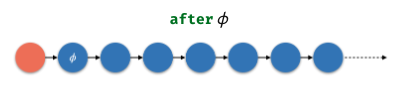
\includegraphics[width=0.6\linewidth]{img/alloy_after.png}
    \caption{$after$ behavioural representation.}
    \label{fig:alloy-after}
\end{figure}

In order to provide a proper contextualization over these concepts, it is desirable to recall the \textit{Eulerian} circuit example. The process of visiting nodes must be specified as it confers the main functionality within the graph theory. It follows the \textit{traverse} predicate to effectively express the latter process. 

\begin{lstlisting}[title={\textit{Eulerian} visiting event.}, otherkeywords = {pred, some, \:, \., not, in, ', \=, \+, \-\>}, floatplacement=H]
pred traverse {
    some adjn : Euler.adj {
        adjn not in Euler.visited
        visited' = visited + Euler->adjn + adjn->Euler
        Euler' = adjn
    }
}
\end{lstlisting}

The first guard states the existence of some node \textit{adjn}, that must be related to the \textit{Euler} node ($Euler \cdot adj$). Another guard is specified to cover the \textit{Eulerian} condition where each edge must be visited exactly once ($adjn\ not\ in\ Euler \cdot visited$). It is followed by \textit{2} effects, where the \textit{visited} relation must account the latest visited edge, and the \textit{Euler} node must be incorporated in the respective adjacent node, within the next state.

\begin{lstlisting}[title={\textit{Eulerian} stutter event.}, otherkeywords = {pred, ', \=}, floatplacement=H]
pred stutter {
    visited' = visited
    Euler' = Euler
}
\end{lstlisting}

Unexpected behavior can occur if no constraints are set on how the system grows through such mutable expressions. Constraints imposed on mutable expressions that should remain unchanged in the next state are referred as \textit{frame conditions}, a formula with primes ($'$) stating the "no change" effect \cite{alloy-docs}.

It is advisable to consider the "nothing changes" possibility in the evaluation of the trace evolution. The \textit{stutter} predicate captures the "no effect" reasoning approach about the behaviour of the system, where frame conditions formulas are enclosed between braces.

Every conceivable trace inside the system must be a permutation of these event handlers performed on a well-defined initial state. When used consistently, this approach constitutes a model design pattern called as Implicit Operation Idiom \cite{gheyi2007formally}.

\begin{lstlisting}[title={\textit{Eulerian} Initial State.}, otherkeywords = {pred, ', \=, no}, floatplacement=H]
pred _init {
    Euler = Init
    no visited
}
\end{lstlisting}

The \textit{\_init} states valid conditions valid in the first state. Thus, to properly specify the initial behaviour of our intended model, every edge must start unvisited ($no\ visited$) and the \textit{Euler} node should start in the \textit{Init} node.

As previously claimed, to reason about state transition, the notion of an execution trace should be duly introduced. The system's permissible behavior will be thoroughly specified by restricting the set of valid operations. As it already been specified every acceptable operation, it is presented the following $fact$ axiom. 

\begin{lstlisting}[title={Trace constraint through the use of an axiom.}, otherkeywords = {fact, ', \=, no, eventually, in\ , and, always, or}, floatplacement=H]
fact traces {
    _init
    always (move or stutter)
}
\end{lstlisting}

The temporal operator $always$ followed by the desired formula is used to impose a state constraint, that must hold one of the \textit{2} events, over the full trace evaluation. This axiom, as explained, must account the initial state (\textit{\_init}) conditions.

The notion of reusable expressions ($fun$) and model assertions ($assert$), are also conceptually included in the Alloy's event idiom. This idiom flexibility allows the developer to define action hierarchy, alongside with sharing atoms passed as parameters, resulting in simpler way of managing specifications \cite{lwspecification, alloy-docs}.


\section{Structural Analysis}

Structural modelling only confers a conventional way of formally expressing the intended behaviour over a software component. To perform verification over the specified behaviour, it is advisable to implement analysis techniques, while supporting an illustrative way of exploring the behaviour through simulations. 

Following the temporal logic semantics, Alloy specification language embeds the linear temporal logic into the first-order logic, thus, it makes use of both temporal and relational quantifiers to properly express behavioural verification over time \cite{lwspecification}. \textit{First-Order Temporal Logics} present additional techniques for reasoning about behaviour, while accounting the basis of the first-order logic, that usually confers the capability to express the well-formedness of the system structure \cite{lwspecification, konur2010survey}.

This section aims to explain how Alloy conducts system analysis, with further explanations over the corresponding analysis commands, along with an overview on the Alloy Analyzer interactive exploration over a system's design. 

\subsection{Analysis and Verification}

Alloy specification process does not establish a clear process separation over the model design and model analysis. This implies that analysis over model checking also accounts the model itself as a combination of properties specification. 

The specification language holds \textit{two} analyzing commands, $run$ and $check$ respectively, as shown above in \textit{Alloy's syntax}. A \textit{First-Order Linear Temporal Logic} (FOLTL) formula is enclosed between braces, to be checked over. Upon executing, both commands accounts the enclosed formula $\psi_{f}$ and the model declaration ${M}$. Likewise in $fact$ declaration, several logic constraints can be combined into the formula $\psi_{f}$. Due to Alloy's implicit abstraction, both commands addresses the relational model specification as truth holder, with the latter being consisted by declarations over $fact$ and $sig$. 

Briefly speaking, $run$ instruct the model-checker to present an example that satisfies the considered formula $\psi_{f}$ over the model definition. This means that the following formula ($M \wedge \psi_{f}$) is expected to hold. The consistency of the \textit{facts} and \textit{signatures} is consequently verified since the model declaration $M$ is also considered. 

Alloy makes use of the $check$ command to perform automatic verification over an $assertion$ declaration. The assertion $\psi_{f}$ verification is done over proving if the following satisfiability formula $M \models \psi_{f}$ is valid within the defined scopes. % while it accounts the declared \textit{facts} as truth holders. 

As result of the first-order logic's undecidability problem, the consistency proofness over satisfiability formulas is not possible \cite{vakili2012temporal}. To ensure decidability, the Alloy Analyzer performs analysis over \textit{scopes}, assigned to each signature declaration. By default, if no scope is provided, the model-checker will account at most \textit{three} atoms for each signature, upon trying to provide an \textit{instance} that satisfies the former formula, consequently proving the behaviour specification (\textit{facts} considerations) consistency. Also, as scopes imposes a limit on the state space of an Alloy model, if no $run$ instance is returned, the formula can not be perceived as inconsistent, as scopes can not be properly set to satisfy the latter.

\begin{figure}[H]
    \centering
    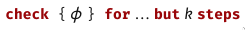
\includegraphics[width=0.4\linewidth]{img/check_alloy_1.png}
    \caption{FOLTL formula $\psi$ verification using \textit{check}, accounting the \textit{Bounded} model checking technique.}
    \label{fig:alloy-check-1}
\end{figure}

Being SAT-based \cite{lwspecification}, the Alloy Analyzer tries to search for a \textit{lasso trace} instance that satisfies the formula $M \models \psi_{f}$ over the \textit{check} command, it performs the latter refutation ($(M \wedge \neg \psi_{p})$ by applying \textit{De Morgan's laws}), yielding a counter-example if the latter is satisfied. This technique is called \textit{Proof by Refutation}: $M$ entails $\psi_{p}$, denoted by $M \models \psi_{f}$, \textit{if and only if} $(M \wedge \neg \psi_{p})$ is unsatisfiable, reducing validity to unsatisfiability.

\begin{figure}[H]
    \centering
    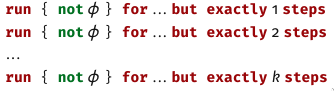
\includegraphics[width=0.5\linewidth]{img/check_alloy_2.png}
    \caption{Reducing Validity to Unsatisfiability.}
    \label{fig:alloy-check-2}
\end{figure}

Moreover, Alloy yields a command to specify the finite number of different steps, related to the expected instance's evaluation trace. This is due to the bounded nature of the Alloy transitions between states, where the \textit{Bounded Model Checking} is considered as model-checking technique. The number of steps is set to \textit{10} by default, although this may be adjusted using the keyword $steps$, alongside with the bounded scopes specification. 

The following $run$ example makes use of both scopes and steps definitions. Moreover, the formula specified in the $run$ states the expected behavioural representation of an \textit{Eulerian} circuit. The $eventually$ (Figure \ref{fig:alloy-eventually}) operator is considered to specify the desired final state, where every edge is visited and the \textit{Euler} node finishes where it started.

\begin{lstlisting}[title={Bounded Model Checking: Eventually the graph will represent an \textit{Eulerian} circuit.}, otherkeywords = {run, eventually, in, and, for, exactly, \5, steps}, floatplacement=H]
run example {
    eventually (adj in visited and Euler in Init)
} for exactly 5 Node, exactly 5 steps
\end{lstlisting}

This particular $run$ yields no instance, so its corresponding formula $M \wedge \psi_{p}$ does not hold, since imposing \textit{5} steps is not sufficient to provide an instance where the desired state, defined by the latter formula, is reached.


\subsubsection{Behavioural Properties}

The verification process over \textit{Model Checking}, needs to account the formal specification of properties that are relevant to reason about the system's temporal behaviour \cite{baier2008principles} .

Alloy makes use of the relational logic (Figure \ref{fig:alloy-rel}) to ensure the well-formedness of the system, which falls short when it comes to supplying support over temporal behaviour. Thereby, Alloy includes temporal connectives from FOLTL semantics, that acknowledges the system's states along the trace evolution \cite{lwspecification, alloy-6, 9341085}.

Ensuring the correctness of a system's behaviour relies on verifying properties regarding the latter's \textit{Safety} and \textit{Liveness}. Its verification technique is motivated by distinct approaches \cite{kindler1994safety}. The former requires an invariance argument, where the latter requires a well-foundedness argument to prove its system satisfiability \cite{alpern1987recognizing}.

A \textit{safety property} asserts that "nothing bad should happen" during the system execution, meaning that, every trace state is expected. Consequently, if a trace that jeopardizes a safety property is found, it can be assumed that the latter has a "bad" property prefix. 

\begin{lstlisting}[title={\textit{Safety Property}: The relation visited can only evolve through time.}, otherkeywords = {always, assert, module, set, fact, iden, no, in, \=, \*, \+, \~, \-\>, \&, '}, floatplacement=H]
assert safety_visited {
    always visited in visited'
} 
\end{lstlisting}

\begin{lstlisting}[title={\textit{Safety Property}: If a node is visited, then once \textit{Euler} was 'inside' it.}, otherkeywords = {always, assert, module, set, fact, iden, no, in, \=, \*, \+, \~, \-\>, \&, all, \:, \., implies, once}, floatplacement=H]
assert safety_euler {
    always (all n :  Node | n in Node.visited implies once Euler = n)
} 
\end{lstlisting}

\begin{figure}[H]
    \centering
    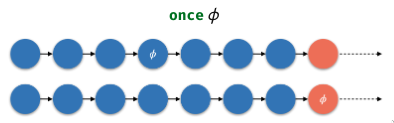
\includegraphics[width=0.6\linewidth]{img/alloy_once.png}
    \caption{$once$ behavioural representation.}
    \label{fig:alloy-once}
\end{figure}

Whereas, a \textit{liveness property} expresses that "something good will happen", implying the eventual occurrence of a state during the course of the system's execution \cite{lamport1977proving}.

\begin{lstlisting}[title={\textit{Liveness Property}: Eventually the graph will represent an \textit{Eulerian} circuit.}, otherkeywords = {assert, eventually, in, and}]
assert liveness_euler {
    eventually (adj in visited and Euler in Init)
} 
\end{lstlisting}

\begin{figure}[H]
    \centering
    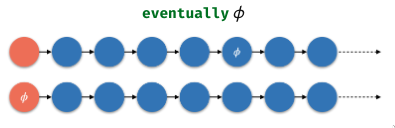
\includegraphics[width=0.6\linewidth]{img/alloy_eventually.png}
    \caption{$eventually$ behavioural representation.}
    \label{fig:alloy-eventually}
\end{figure}

The above-mentioned properties make use of \textit{2} relevant over time quantifiers. The $once$ operator expresses the past validation of a given formula. The $eventually$ operator expresses an existence quantifier, imposing the formula verification somewhere along the trace evolution \cite{alloy-docs}.

Moreover, the liveness property states the expected behavioural representation of an \textit{Eulerian} circuit, where the $eventually$ (Figure \ref{fig:alloy-eventually}) operator is considered to specify the desired final state. However, its verification, using $check\ liveness\_euler$, yields a counterexample, as it is possible to always perform the \textit{stutter} event, and thus the expected behaviour never happens. This scenario results in an implausible infinite trace behavior, which must be handled by adding fairness to the trace assessment. 

Liveness properties evaluation process reasons about states that eventually might reach the wanted scenario. Then, it is advisable to consider \textit{fairness} constraints, intentionally specified to rule out infinite traces with unrealistic behaviour, such as system stuttering \cite{baier2008principles}. Briefly, a \textit{fairness} constraint imposes fairly considerations on the system's trace evolution \cite{wahlfairness}.

\begin{lstlisting}[title={\textit{Fairness predicate}: If \textit{Euler} has an adjacent node, it will eventually visit the latter.}, otherkeywords = {pred, eventually, always, implies, some, \.}]
pred fairness {
	(eventually always some Euler.adj) implies (always eventually traverse)
}
\end{lstlisting}

The latter imposes a fairness constraint regarding the trace evolution, ensuring that trace stuttering is not possible as long as the \textit{Euler} node has some adjacent node that is not been visited yet. As expected, by instructing the Analyzer to check the asserted property ($check\ liveness\_euler$), it will return no counterexample.

\begin{lstlisting}[title={\textit{Liveness} property accounting the fairness constraint. It yields no counterexample.}, otherkeywords = {assert, in, and, eventually, check}]
assert liveness_euler {
	fairness implies eventually (adj in visited and Euler in Init)
} check liveness_euler
\end{lstlisting}

\subsection{Alloy Analyzer}

Normally, the specification process upon abstracting the system as a conventional model is carried out interactively, since considerations about model validation must be preceded by the model specification. The already mentioned analysis techniques, $run$ and $check$ analysis commands respectively, instruct the Analyzer to check and provide analysis over their implicit formula nature. 

Moreover, the Analyzer is capable of providing model instances concerning the formula evaluation, depicted graphically as graph-like structures, through the usage of the Alloy \textit{Visualizer}. The latter allows instance interaction over multiple configuration buttons. Additionally, concerning the user comprehension, the graphical depiction of these instances can be customized using \textit{Themes}, through the \mybox{Theme} toolbar button.

Recall the $run$ example that failed to provide a model instance due to the $steps$ explicit limitation. To find an \textit{Eulerian} circuit instance for $n$ nodes, the minimum of $n+1$ steps are required.

\begin{lstlisting}[title={Bounded Model Checking: Eventually the graph will represent an \textit{Eulerian} circuit.}, otherkeywords = {run, eventually, in, and, for, exactly, \5, steps}, floatplacement=H]
run example {
    eventually (adj in visited and Euler in Init)
} for exactly 5 Node
\end{lstlisting}

Producing a concrete instance might be quite helpful throughout the modeling process. The $run$ command presented above is capable of providing a model instance as it performs Bounded Model Checking for at most \textit{10} steps. The Analyzer executes the command and generates an instance regarding the latter, consequently producing a visual graphical (Figure \ref{fig:alloy-valid-run}) through the usage of the Visualizer.

\begin{figure}[H]
    \centering
    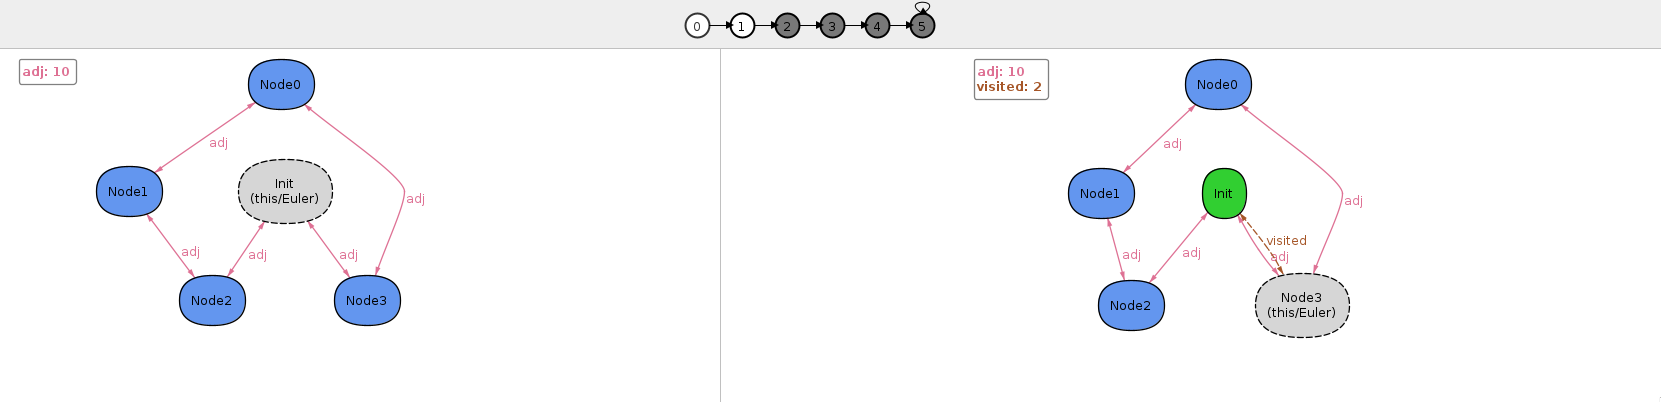
\includegraphics[width=\linewidth]{img/alloy_run.png}
    \caption{Partial graphical view of the \textit{two} initial states. The \textit{Euler} node starts in the \textit{Init} node, and then moves towards an adjacent node.}
    \label{fig:alloy-valid-run}
\end{figure}

The Visualizer furnishes a toolbar with multiple configuration buttons, allowing interactive customization over alternative instances \cite{alloy-docs}. Traces can also be interactively overviewed through transition buttons ($ \rightarrow $ and $ \leftarrow $), enabling forward and backward trace navigation.

\begin{figure}[H]
    \centering
    
\includegraphics[width=0.7\linewidth]{img/alloy_buttons.png}
    \caption{Alloy Visualizer toolbar.}
    \label{fig:alloy-toolbar}
\end{figure}

The \mybox{New Config} instructs the Analyzer to provide a new trace configuration, where immutable model expressions (sets and relations) are depicted with new values. Consequently, the Visualizer will present an execution trace regarding the new model configuration. The \mybox{New Trace} instructs the Analyzer to present a new execution trace, regarding the same model configuration. The \mybox{New Init} requests for a new trace representation, where the initial state is forced to present different model expressions values. At last, the \mybox{New Fork} allows alternative transition behaviour exploration over the same starting state, depicting a new transition post-state. The latter could differ on the result of a given event, or it can display the outcome of a different event \cite{alloy-docs}.

Alloy forces the property formula translation into an LTL-based formula, considering the finitude of its universe of comprehension. Due to the emphasis on representing instances over infinite traces, every Alloy instance generated by the Analyzer, captures an infinite trace through \textit{lassos}, where a looping state is reached.

Concerning performance in the evaluation over infinite traces, Alloy considers the Bounded Model Checking technique as the first approach towards the model verification. Here, the corresponding formula is verified for all \textit{lasso} traces of size up to a bounded number of steps. So, the verification is not complete, due to the SAT time-bounded nature. However, it still confers great functionality, as infinite traces can often be represented as finite traces, making verification within small scopes possible \cite{jackson2012software}.

\begin{figure}[H]
    \centering
    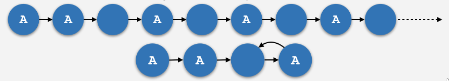
\includegraphics[width=0.7\linewidth]{img/alloy_infinite_trace.png}
    \caption{Some infinite traces can be represented by finite \textit{lasso} traces.}
    \label{fig:alloy-infinite}
\end{figure}

Oppositely, the Analyzer can be instructed to perform \textit{Unbounded Model Checking} towards achieving consistency over model verification, without bounding traces upfront \cite{alloy-6, alloy-docs}. This is feasible as the state space is finite due to the Alloy analysis way of bounding signatures. Consequently, it constrains infinite traces as periodic \textit{lasso} traces (Figure \ref{fig:alloy-infinite}).

To perform complete model-checking, an appropriate solver must be selected in the \mybox{Options} menu, and the time scope must be specified under the following syntax: $for\ 1..\ steps$. Consider the previous $run$ command in terms of the Unbounded Model Checking approach. 

\begin{lstlisting}[title={Unbounded Model Checking: Eventually the graph will represent an \textit{Eulerian} circuit.}, otherkeywords = {run, eventually, in, and, for, exactly, \5, steps}, floatplacement=H]
run example {
    eventually (adj in visited and Euler in Init)
} for exactly 5 Node, 1.. steps
\end{lstlisting}

\section{Related Work}\label{s:relWork-pv}

As reliance on robotic systems grows due to their expanding application across a wide range of domains, these systems concern critical scenarios, where human interaction comes in hand \cite{diluoffo2018robot}. Thus, security should be highly considered upon employing systems that might jeopardize the human's integrity, such as robotics. Additionally, ensuring analysis regarding the system's quality assurance is increasingly becoming a focus of attention. Consequently, it is critical to employ techniques that promote the increase of the system quality, without sacrificing its flexible nature.

\citeauthor{cortesi2013static} in \textit{Static Analysis Techniques
for Robotics Software Verification} \cite{cortesi2013static} gives a proper understanding on how important it is to perform formal analysis to ensure  the reliability of the resulting software, while significantly minimizing the testing effort. Here, the authors intend to cover multiple static analysis techniques to properly contextualize robotic developers about which is the most appropriate analysis strategy to follow based on the kind of examined property and software system. After briefly introducing to each technique, the authors present an overall evaluation of the various static analyzes techniques, following several criteria: automation, precision, scalability, and soundness. \citeauthor*{cortesi2013static} conclude stating that performing analysis techniques is highly fundamental to develop robotics software. Additionally, the authors discuss the difficulties of guaranteeing adequate automated analysis of complex properties. Finally, they emphasize the need of future reasearch within this formal verification context, due to its role in software development. 

This section concerns the study of some relevant studies that introduces to some pertinent quality assurance procedures over the robotics domain. The latter's concentration will be on the following subjects: First, system analysis regarding static procedures will be contextualized, emphasizing a notable framework, called \textit{HAROS}, that performs static evaluation over ROS-based applications; After that, various state-of-art methodologies based on property verification are given as support to this dissertation analysis approach.

Even though this dissertation was devoted to a detailed examination of ROS framework regarding its security deployment, there is no obvious line separating the ROS difficulties from those of other popular multi-configurable robotic software in terms of quality assurance and security overview. As result, a broader range of robotic systems will be explored to give contextualization of some relevant aspects that also fall under the ROS domain.

Analysis through property verification in the ROS framework represents a major contribution to this dissertation domain, in which researchers aim to tackle issues arose from miss configurations or code inconsistencies. Although researches and tools on analysis of ROS systems are scarce, there are some presented work that might be useful within the context of this dissertation.

For instance, a natural way of performing analysis over a system is by observing the communication architecture. Recall that the Alloy Visualizer is useful to observe the system behaviour as traces through state evaluation. Here, ROS provides a framework for GUI development plugin called \textit{rqt\_graph} \footnote[2]{http://wiki.ros.org/rqt\_graph}, in which ROS developers usually rely on. It is used to depict the network architecture through a graph with run-time statistics. However, this approach lacks on providing trustworthy analysis over more complex networks, where features such as security control are implicit.

The noteworthy \textit{HAROS} framework, initially proposed by \citeauthor{santos2016framework} in \textit{A framework for quality assessment of ROS repositories} \cite{santos2016framework}, holds great value thanks to its contribution in improving ROS's software quality. \textit{HAROS} makes use of several analysis techniques to exert quality evaluation of ROS software, followed by ways of feed-backing inconsistencies using predefined code metrics. As this framework seeks to be flexible when it comes to adding functionality, further static analysis works improvements have been proposed as plugins.

In both \citenum{santos2019static} and \citenum{santos2018property}, it is presented additional functionality to the framework, through applying architectural considerations over metamodel designing, where the latter supports the former by supplying property-based specifications. These techniques confers great help back to developers, since static analysis offers advantageable usage over raw review of software code. 

The literature concerning property verification has already been explored through state-of-art model checkers, where safety properties regarding the robotics domain were studied and verified. Within the ROS context, certain techniques were proposed that primarily focused on modeling the ROS node-communication, while real-time properties were also considered as support to the target language.
 
Within this context, \citeauthor*{halder2017formal} provides a model-based approach to reason about the communication between nodes in ROS-based systems, emphasizing the specification of real time properties. Here, the authors apply model techniques over ROS applications, abstracting them as timed automatas. Property verification is then ensured by model checking through the \textit{UPPAAL} \footnote[3]{https://uppaal.org/} model checker. 

Notably, this work provides a brief introduction to the concepts of timed automata and their implementation into \textit{UPPAAL}, with respect to the latter's temporal logic as a query language to describe desired properties. After contextualizing the code behind a ROS-based application, the authors proceed to perform model checking using the source code of a popular physical robot \textit{Kobuki} \footnote[4]{http://kobuki.yujinrobot.com/}. This allowed the authors to reason about context specific properties of the latter, aside from the safety properties.

\citeauthor*{halder2017formal} conclude their work by emphasizing the importance of model-checking in finding and checking these desirable properties, stating if only physical verification was considered, the latter's properties would be extremely difficult, time-consuming or infeasible to find.

A noteworthy study is supplemented by \citeauthor*{white2019network}, in \textit{Network Reconnaissance and Vulnerability Excavation of Secure DDS Systems} \cite{white2019network}. \citeauthor{white2019network} continues to address security \cite{white2016sros, white2018procedurally} through an alternative approach. Here, the author makes use of formal verification and model checking to reason about reachability of information flow, related to an attack model that studies the network through targeted attacks. This study starts to overview the DDS security protocol and its model, to make further speculations about the lack of support for some additional security threats from the latter. 

Within this scenario, \citeauthor{white2019network} intends to explore the data flow semantics to address the DDS networks vulnerability. After conceiving the threat model, some attack assumptions are explicitly defined over the attack model. Unlike previous network reconnaissance methods and considering the assumptions discussed in the attack model, this approach allows an attacker to build the topology through a graph based database by passively sniffing packets inside the network. This database is then made available to the SAT solver in order for it to compute queries. \textit{Imandra} \footnote[5]{https://www.imandra.ai/} model checking tool is then used as SAT solver by replicating the DDS security protocol functionalities (especially the access control) as functional models, to accurately represent default plugin logic. Thus, the attack model assumptions can be then specified over SAT queries, allowing the replicated models to reflect a new SAT. Moreover, using formal verification and model checking, vulnerability excavation can be efficiently performed over the inquired graph, instead of engaging with the targeted system. 

The authors conclude their work by reasoning about how crucial is to employ attack models for general system validation. Also, the usage of formal verification techniques can reason about a large state space without exhaustive search.

A remarkable work that duly fits under this dissertation domain of exploration is presented in \citenum{9341085}. Here, \citeauthor{9341085} presents a notable proposal to automatically verify system-wide properties of ROS applications at static time, emphasizing their safeness behaviour. Here, the authors intend to abstract each application behaviour through concrete models, to then perform model-checking over system-wide specifications, using \textit{Electrum} as model checker. 

In order to integrate analysis of ROS-based applications, the authors make use of the already mentioned \textit{HAROS} plugin-based framework, that provides quality assessment of ROS software. \textit{HAROS} allows the automatic extraction of the system structure based-on an architectural model, based on a static analysis of the source code. Then, using a domain-specific property-based language, it allows reasoning about the specialist's system behavior. 

\begin{figure}[H]
    \centering
    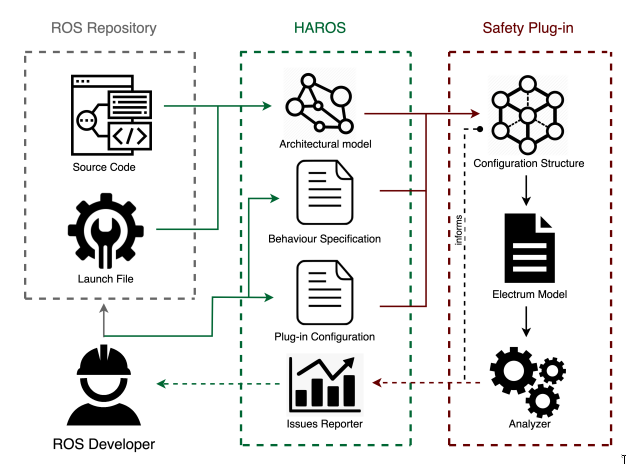
\includegraphics[width=0.6\linewidth]{img/haros-electrum-plugin.png}
    \caption{Architecture of the \textit{HAROS} safety plugin for ROS. Extracted from \cite{9341085}.}
    \label{fig:haros-electrum}
\end{figure}

The safety plugin denotes the backend of the depicted architecture (Figure \ref{fig:haros-electrum}), where it relies on \textit{Electrum}, the former version of the current \textit{Alloy Analyzer}, to model and reason about the application behaviour through properties expressed in FOTL. Afterwards, the authors pretend to extend \textit{HAROS}' functionality by offering a plugin that automatically converts \textit{HAROS} artifacts into \textit{Electrum}. Additionally, the framework reports model checking counter-examples in a more user-friendly manner via its quality reporting interface. 


Through ROS launch configurations, the plugin automatically generated models using Electrum and performs verification over these models, to then feedback issues related to their ROS system behaviour.

As ROS2 domain regards the use of DDS communication protocol, a few works on DDS modelling analysis deserve to be mentioned, as they might give important background for property verification over communications protocols. In \citenum{alaerjan2017modeling}, it is proposed a technique to model the DCPS architectural design that DDS makes use of, alongside with new approaches to the current DDS behaviour. Supported by several modelling techniques for publish-subscribe systems, in \citenum{liu2018formal}, DDS in ROS2 is formalized as a timed automata, consequently followed by model verification over property-checking. These works conceive value concepts and procedures useful for this dissertation contextualization.

A few studies on robotics should be recognized in which techniques such as model-checking were performed. Despite the fact that they do not address the domain of ROS, they nonetheless give helpful background for the robotics research over formal approaches. 

A case study, mentioned in \citenum{near2011lightweight}, presents a novel approach over systems that require static analysis based on software assumptions and proper analysis within its environment usage, where user-interaction comes in hand. Concerning this novel idea, a medical system is concerned as a case study, where multiple safety-based considerations are expected, as well as, an end-to-end critical property that must be satisfied over the entire analysis course. 

Another notable work regarding former analysis using Alloy specification language is presented in \citenum{mansoor2018modeling}, where a safety-critical scenario is proposed under the domain of surgical robots. The formal techniques used allows overview over a surgical robot arm, taking into consideration possible violations of important safety properties. 

Although these studies presents favorable outcomes, their focus lies on a particular area of study. As a result, they lack on providing solutions to a vast majority of situations.